%%
% このファイルは、卒業論文の本文テンプレートです。
% sample-jp-utf8 と同様の書式で執筆できます。
%
% 必要に応じてタイトル・著者・指導教員などを書き換えてください。
%%
\documentclass[a4paper,11pt]{jreport}

%% 画像貼り込み
\usepackage[dvipdfmx]{graphicx}
\usepackage{placeins}
\usepackage{times}

\setcounter{tocdepth}{3}
\setcounter{secnumdepth}{3}
\setcounter{page}{-1}

\setlength{\oddsidemargin}{0.1in}
\setlength{\evensidemargin}{0.1in}
\setlength{\topmargin}{0in}
\setlength{\textwidth}{6in}
\setlength{\parskip}{0em}
\setlength{\topsep}{0em}

%% タイトル生成用パッケージ
\usepackage{mast-jp-utf8}

%% タイトル情報
\title{複数の小型プロペラを用いた力覚提示の方向知覚特性の調査}
\author{石井 晃斗}
\advisor{川口 一画，志築 文太郎}
\majorfield{　} \yearandmonth{2026年 2月}

\begin{document}
\maketitle
\thispagestyle{empty}
\newpage

\thispagestyle{empty}
\vspace*{20pt plus 1fil}
\parindent=1zw
\noindent

%% 概要（Abstract）
\begin{center}
{\bf 概要}
\vspace{5mm}
\end{center}
　スマートウォッチなどの小型デバイスを用いた方向提示は，道案内などの場面で活用されている．現在，スマートウォッチ等で一般的に用いられている方向提示手法は，短い振動の回数やパターンで方向を符号化する方法，あるいは瞬間的な触覚提示に依存する方法が多く，提示できる方向数が限られる，あるいは解釈のための認知負荷が高いといった課題がある．一方，より大型の装置では持続的な力覚による分かりやすい方向提示を実現することが可能であり，例として盲導犬ロボットや圧縮空気噴射デバイスを用いる手法が研究されている．しかし，これらは強力な力覚を発生させるために大型の装置を要し，小型デバイスへの実装には適さない．そこで本研究では，小型デバイスで力覚による方向提示を実現するため，ドローン用の小型プロペラを用いた力覚提示手法を提案する．本研究では，2種類の装着方式からなる，複数の小型プロペラを組み込んだ力覚提示デバイスを用いて提示方向の知覚特性を調査した．調査の結果，プロペラによる方向提示を行うデバイスにおいては，装着方式が知覚特性と負荷に大きく影響することが示唆された．

\par
\vspace{0pt plus 1fil}
\newpage

\pagenumbering{roman}
\tableofcontents
\listoffigures
\listoftables

%% 本文開始
\pagebreak \setcounter{page}{1}
\pagenumbering{arabic}

\chapter{はじめに}
本研究では，複数のドローン用小型プロペラを用いた方向を伴う力覚提示デバイスを提案する．さらに，提案システムを用いた実験を実施し，装着方式が提示方向の知覚特性に与える影響を調査した．本章では，本研究の背景として，既存の方向提示手法の知見および課題を説明する．次に，本研究の目的とアプローチ，貢献，および本論文の構成を示す．

\section{背景}
スマートウォッチなどの小型デバイスを用いた方向提示は，道案内などの場面で活用されている．現在，市販品のスマートウォッチ等では，右や左などの方向に対応する複数の振動のパターンを用いた方向提示を行っている．その他にも，小型デバイスを用いて方向提示を行う手法として，振動デバイスを利用して瞬間的な触覚提示を行う手法は多く研究されている\cite{stock2020feedi}\cite{ntt_burunavi4}．しかし，これらのような瞬間的な振動触覚を活用した方向提示には，提示できる方向数が限られる，あるいは解釈のための認知負荷が高いといった課題が考えられる．

一方，より大型の装置では持続的な力覚による分かりやすい方向提示を実現することが可能であり，例として盲導犬ロボット\cite{cai2024rdog}や圧縮空気噴射デバイスを用いる手法\cite{ma2024airpush}が研究されている．しかし，これらは強力な力覚を発生させるために大型の装置を要し，小型デバイスへの実装には適さないという課題が存在する．力覚提示デバイスに関する研究の多くはVRなどの体験向上を目的としたものであり，屋外で携帯可能な大きさの小型デバイスに関する研究は少ない．そこで本研究では，小型デバイスで力覚による方向提示を行った際の知覚特性を調査することを目的とし，ドローン用の小型プロペラを用いた力覚提示手法を提案する．

\section{目的とアプローチ}
本研究の目的は，小型デバイスで力覚による方向提示を行った際の知覚特性を調査することである．先行研究で実装されている力覚提示デバイスの多くでは，力覚フィードバックによる触覚再現を目的としていることから，方向提示のみを目的とした，最小構成の力覚提示デバイスに関する知見は限られている．

そこで本研究では，ドローン用の小型プロペラを複数搭載した力覚提示デバイスを設計・製作した．このデバイスは，4つのプロペラを円周上に配置し，各プロペラの駆動によって特定の方向から持続的な空気力を提示することが可能である．また，装着方式による違いを評価するため，手首装着型および手持ち型の2種類の筐体を試作した．このデバイスを用いて，小型デバイスで力覚による方向提示を行った際の知覚特性を調査するとともに，装着方式が知覚特性と負荷に与える影響を評価する．

\section{貢献}
本研究の貢献は以下の通りである．
\begin{itemize}
    \item ドローン用の小型プロペラを用いた小型デバイスによる力覚提示手法を提案した．
    \item 提案システムを使用した力覚による方向提示を行った際の知覚特性を調査した．
    \item 装着方式が知覚特性と負荷に与える影響を評価した．
\end{itemize}

\section{本論文の構成}
本論文の構成を述べる．第1章においては，本研究の背景，目的とアプローチ，および貢献を示した．第2章においては，本研究に関連する研究を述べ，本研究の位置づけを示す．第3章においては，本研究における提案システムを示す．第4章においては，本研究を評価するために行った評価実験について述べる．第5章においては，4章において述べた実験における結果，および考察を述べる．第6章においては，本研究における制約および今後の課題を述べる．第7章においては，本研究の結論を述べる．

\chapter{関連研究}
本章では，これまで行われてきたナビゲーションや方向提示に関する研究を提示し，力覚提示による方向提示を行うことでどのような利点があるかを述べる．その後，力覚提示を行うデバイスに関する研究を提示し，本研究の位置づけを示す．

\section{大型装置によるナビゲーションに関する研究}
大型装置による方向提示手法は，主にナビゲーションなどの用途で多く研究されている．Caiらが提案するRDog\cite{cai2024rdog}は，4足歩行型ロボットを用いて視覚障害者の移動を支援するシステムである．このシステムでは，力覚フィードバックを伴う具体的な経路の誘導を行うことによって，従来の音声のみでの案内を行うデバイスと比較してより効率的なナビゲーションと認知的な負荷の軽減を実現可能であることが示された．また，高田らの研究\cite{takada2019propeller}では，ヘルメットの頭頂部に飛行ドローンを装着することにより，プロペラの推進力によってユーザの頭部を牽引し，ユーザの歩行方向を制御する手法を提案している．この手法を用いることにより，歩行時および静止時に，意図して逆らわないと歩き出す程度の牽引力を提示できることが示されている．

以上のことから，牽引力などの力覚を利用した方向提示手法は，ナビゲーションなどの用途において有効な手法であると考えられる．しかしながら，これらの手法は大型のロボットやドローンを必要とすることから，ウェアラブルデバイスへ直接応用することは難しいと考えられる．

\section{ウェアラブルデバイスを用いた方向提示手法に関する研究}
ウェアラブルデバイスや，携帯可能な小型デバイスを用いた方向提示に関する研究も複数行われている．FEEDI\cite{stock2020feedi}は，足部に装着することで，ナビゲーションや方向提示を行うことが可能なデバイスである．このデバイスでは，8方向にそれぞれ対応する振動モータを搭載し，振動触覚による方向提示を行うことが可能である．そのほかにも，ぶるなび4\cite{ntt_burunavi4}は，非対称振動による錯覚を利用した方向提示デバイスであり，多自由度の方向提示を行うことが可能である．しかし，これらの振動触覚を利用した方向提示手法には，提示できる方向数が限られる，あるいは解釈のための認知負荷が高いといった課題が考えられる．Yuxinらの研究\cite{ma2024airpush}では，振動触覚は質感の表現によく用いられるが，持続的な重みや物体からの反力といった継続的な物理的抵抗を表現するには不十分であることを指摘している．

以上のことから，より質の高い方向を提示するためには，力覚提示を行うデバイスを用いることが有効であると考えられる．

\section{力覚提示を行うデバイスに関する研究}
力覚提示を行うデバイスに関する研究も多数行われている．主にVRの体験向上を目的としたものであり，力覚の発生源としても様々なものが提案されている．AirPush\cite{ma2024airpush}は，指先に圧縮空気を噴射することにより，指先に方向を伴う力覚フィードバックを提示するデバイスである．このデバイスでは，力覚の発生源として接地型のエアコンプレッサを使用している．また，Thor's Hammer\cite{heo2018thorshammer}は，6 つのモータとプロペラを利用して 3 次元の自由な方向に力覚を発生させることが可能なデバイスであり，プロペラを利用した手持ち型のデバイスにより明瞭な方向提示が可能であることを示している．このデバイスでは，力覚の発生源として複数の大型プロペラの回転を利用しており，モータへの電力供給を外部の電源から行っている．

これらの研究は，力覚提示を用いることによりユーザに対して明瞭な方向提示を行うことが可能であることを示している．しかしながら，これらのシステムの研究目的はVRの体験向上を目的としているため，触覚再現のために方向提示としては過剰な強さの力覚を提示する機能を備えている．結果，強力な力覚を発生させるために大型のプロペラや外付けのパワーソースを必要とすることから，これらのシステムを直接ウェアラブルデバイスとして活用することは難しい．しかしながら，ナビゲーション用の方向提示に役割を限定させた，より小
型の動力源とバッテリを備えた小型デバイスを実装することは十分可能であると考えられる．

そこで本研究では，小型デバイスで力覚による方向提示を行うため，ドローン用の小型プロペラを用いた力覚提示手法を提案し，小型デバイスで力覚による方向提示を行った際の知覚特性を調査することを目的とする．

\chapter{提案システム}
本章では，本研究にて用いたシステムの設計を述べる．最初にシステムの設計指針について述べた後，システムの構成について述べる．

\section{設計指針}
2章で得られた知見をもとに，本研究では，手に持つ，もしくは腕に装着可能なほど小型な，力覚提示により方向提示を行うデバイスを提案する．本システムでは，力覚の発生源としてドローン用の小型プロペラを用いることにより，小型デバイスでも力覚による方向提示を行うことが可能である．このシステムを使用することにより，ユーザは力覚による明瞭な方向提示を受けることが可能となることが期待される．

また，力覚を与える体の部位によって提示方向の知覚特性が異なることが考えられる．そこで本研究では，装着方式が提示方向の知覚特性に与える影響を評価することを目的として，手首装着型および手持ち型の2種類の筐体を製作する．

\section{システム構成}
本研究にて製作したシステムは，4つの小型モータをESP32マイコンとMX1508モータドライバで制御する形で実装した．ESP32マイコンは，Bluetooth Low Energy(BLE)を用いて外部のアプリケーションから制御を受けることが可能である．

\subsection{ハードウェア}
本システムでは，4つの直径75 mmプロペラを同一平面上の4方向に配置し，約40000RPMの3.7 Vマイクロコアレスモータで駆動する．このモータを，MX1508モータドライバで制御することにより，モータの回転方向および回転速度を制御することが可能である．4つのプロペラから生じる推力を合成することで，同一平面上の任意の方向に調整可能な力覚を発生させることができる．モータ制御回路の実装図を図\ref{fig:hardware-configuration}に示す．また，デバイスを上から見た際の各モータの配置およびモータ正転時の力覚提示方向を図\ref{fig:motor-direction}に示す．

\begin{figure}[htbp]
\begin{center}
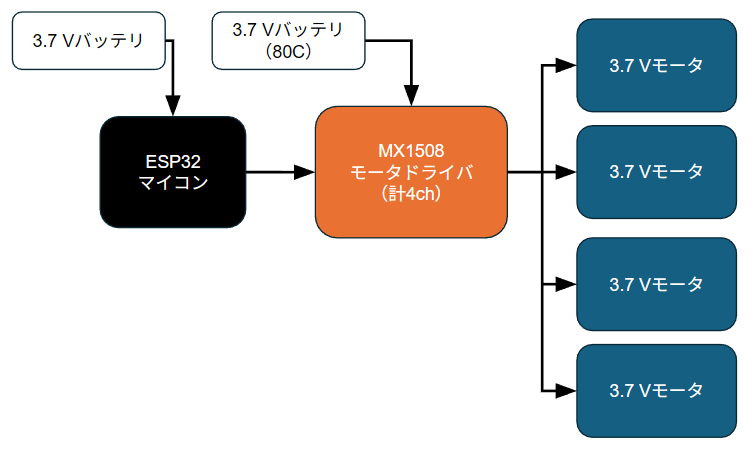
\includegraphics[width=0.85\textwidth]{figure/hardwere-kousei.png}
\end{center}
\caption{モータ制御回路の実装図}
\label{fig:hardware-configuration}
\end{figure}

\begin{figure}[htbp]
\begin{center}
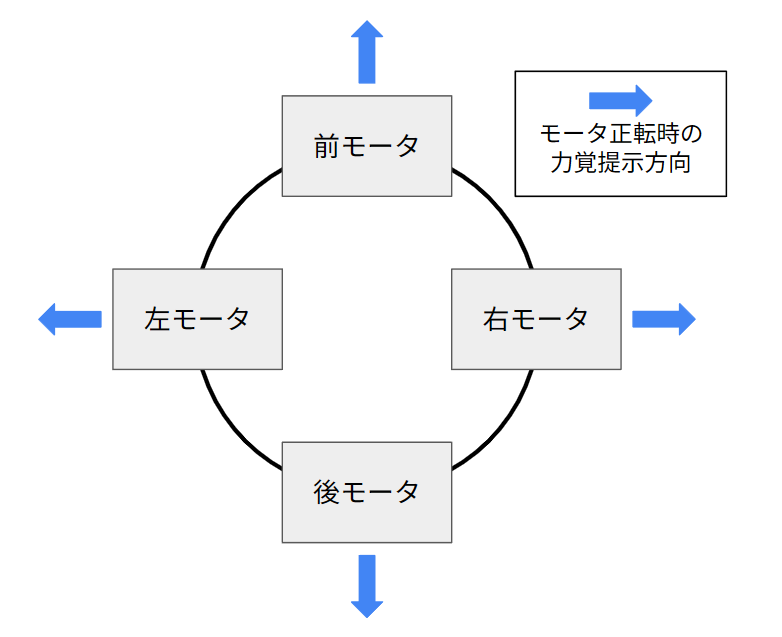
\includegraphics[width=0.55\textwidth]{figure/motor_direction.png}
\end{center}
\caption{デバイスを上から見た際の各モータ配置と正転時の力覚提示方向}
\label{fig:motor-direction}
\end{figure}

\FloatBarrier

本システムの実装においては，マイコンにESP32-DevKitCを使用した．ESP32-DevKitCは，ESP32マイコンを搭載した開発ボードであり，2.4 GHzのWi-FiとBluetoothによる通信機能を内蔵している．また，これらのマイコンおよびモータドライバへの電源供給はそれぞれ独立したリチウムイオンバッテリから行うことにより，デバイスの小型化を実現した．また，モータドライバに接続するバッテリには高Cレートのバッテリを使用することで，全てのモータが高速回転している際にも安定して電力を供給することが可能となっている．これらのバッテリやマイコンなどは充分に軽量かつ小型であるため，先行研究で提案されている力覚提示デバイスの課題点である携帯性の低さを克服している．なお，4章で実施した実験においては，モータ制御回路の一部をブレッドボード上に実装しており，バッテリおよびモータドライバはデバイス本体に格納されていない．

デバイス本体の筐体作成は3Dプリンタを用いて行った．筐体3Dデータの設計にはAutodesk Fusion 360\cite{autodesk_fusion360}を使用している．また，筐体を設計するにあたり，最適なプロペラの配置や筐体の形状を探るため，複数の試作品を作成した．筐体の試作品の一例を図\ref{fig:sample-body}に示す．

\begin{figure}[htbp]
\begin{center}
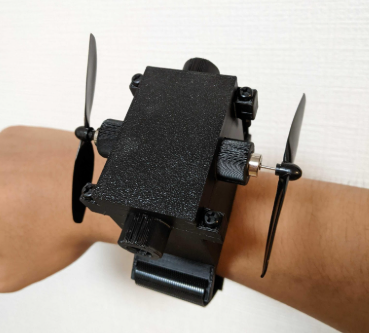
\includegraphics[width=0.85\textwidth]{figure/sisakuhin.png}
\end{center}
\caption{筐体の試作品の一例}
\label{fig:sample-body}
\end{figure}

最終的に，保持する手法が異なる2種類の筐体を製作した．1つは，手首に装着するタイプの筐体であり，もう1つは，手で握るタイプの筐体である．手首に装着するタイプの筐体を図\ref{fig:wrist-worn-body}に示し，手で握るタイプの筐体を図\ref{fig:hand-grip-body}に示す．これらの筐体には回転するプロペラから身体を保護するためのシールドが設けられている．

\begin{figure}[htbp]
\begin{center}
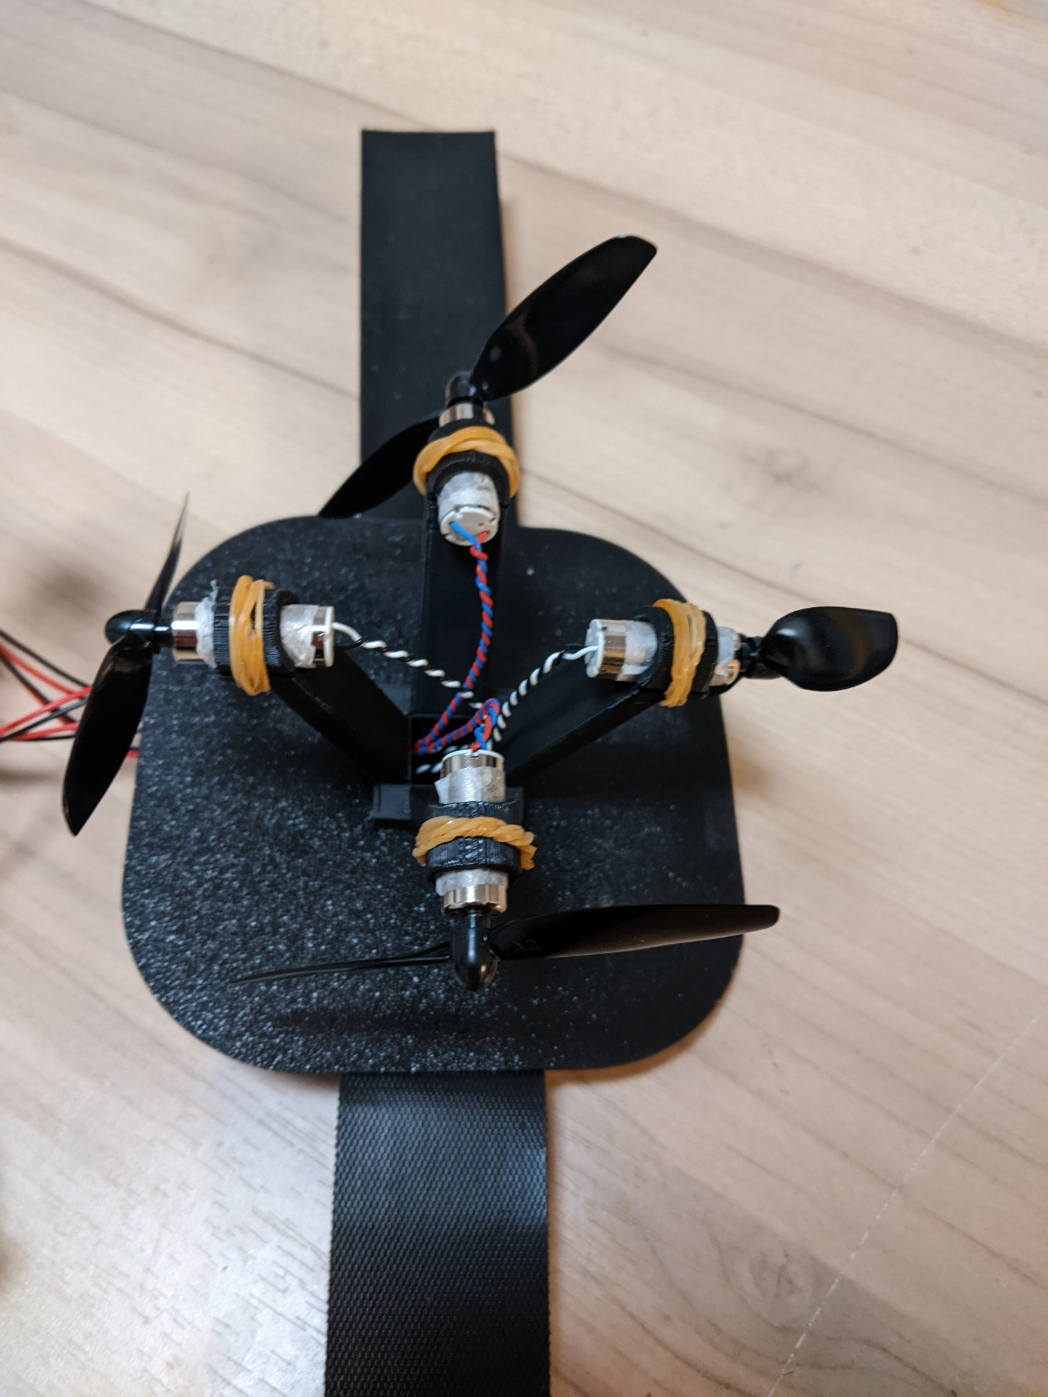
\includegraphics[width=0.85\textwidth]{figure/wrist-worn.jpg}
\end{center}
\caption{手首に装着するタイプの筐体}
\label{fig:wrist-worn-body}
\end{figure}

\begin{figure}[htbp]
\begin{center}
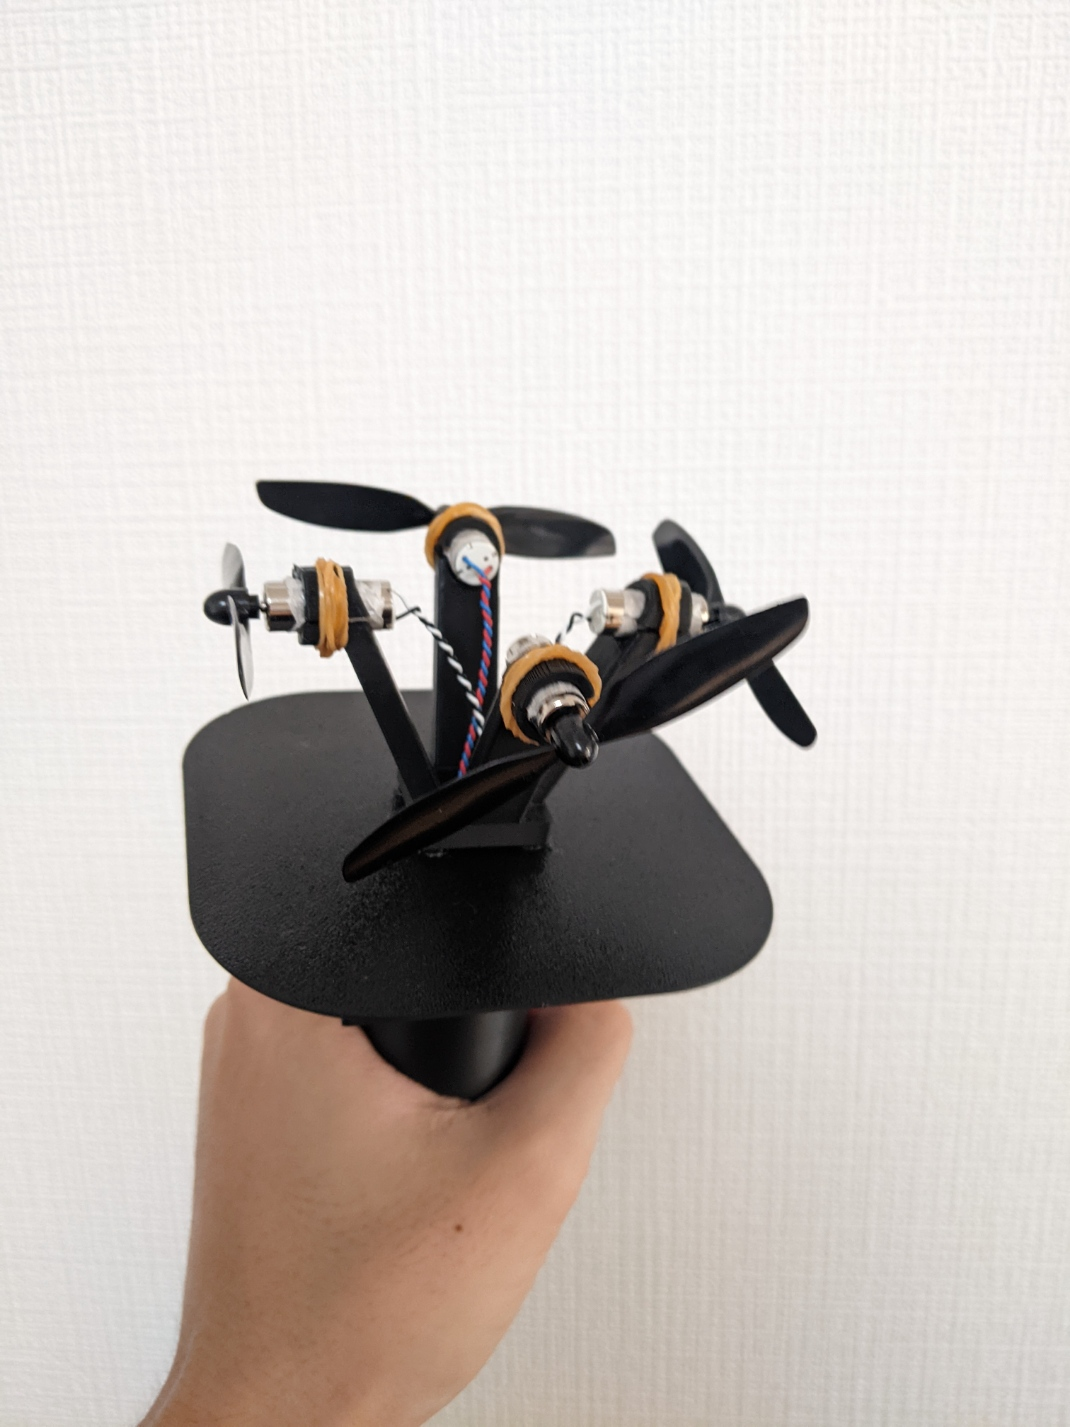
\includegraphics[width=0.85\textwidth]{figure/hand-grip.jpg}
\end{center}
\caption{手で握るタイプの筐体}
\label{fig:hand-grip-body}
\end{figure}

\FloatBarrier

\subsection{ソフトウェア}
本システムでは，ESP32マイコンをArduino言語のプログラムで制御することにより，モータの制御を行う．通信にはBluetooth Low Energy（BLE）を用い，ESP32はBLEペリフェラルとして動作する．送信データはUTF-8テキストとし，角度のみのコマンド（例：`90`）または角度とデューティ比を併記したコマンド（例：`90 75`）を送信する．

4章で実施する実験においては，角度は0，45，90，135，180，225，270，315度の8方向のみを用い，デューティ比は70\%および100\%の2段階で指定可能である．
角度コマンドと各モータ（右A，前B，左C，後D）の回転方向（正転・逆転・停止）の対応を表\ref{tab:angle-motor-direction}に示す．

\begin{table}[htbp]
\begin{center}
\caption{角度コマンドと各モータの回転方向の対応}
\label{tab:angle-motor-direction}
\begin{tabular}{c|cccc}
角度コマンド & 右A & 前B & 左C & 後D \\
\hline
\texttt{0}   & 正転 & 停止 & 逆転 & 停止 \\
\texttt{45}  & 正転 & 正転 & 逆転 & 逆転 \\
\texttt{90}  & 停止 & 正転 & 停止 & 逆転 \\
\texttt{135} & 逆転 & 正転 & 正転 & 逆転 \\
\texttt{180} & 逆転 & 停止 & 正転 & 停止 \\
\texttt{225} & 逆転 & 逆転 & 正転 & 正転 \\
\texttt{270} & 停止 & 逆転 & 停止 & 正転 \\
\texttt{315} & 正転 & 逆転 & 逆転 & 正転 \\
\end{tabular}
\end{center}
\end{table}

実験においては，実験用Webアプリと提案デバイスをBLE経由で通信することによりデバイスの制御を行う．実験用Webアプリの仕様に関しては，4章で詳述する．

\chapter{実験}
本研究では，小型プロペラによる力覚提示による方向知覚特性を調査するため，実装したシステムを用いて実験を行った．本章では，本実験における実験条件，実験タスク，実験環境，実験手順，および評価指標を述べる．

\section{実験条件}
実験条件は以下の2条件で，全て参加者内配置で設計した．

\begin{itemize}
    \item \textbf{wrist-worn条件} 手首に装着するタイプの筐体を使用する．
    \item \textbf{hand-grip条件} 手で握るタイプの筐体を使用する．
\end{itemize}

\section{実験タスク}
\label{sec:experiment-task}
本実験では，提案システムからランダムに提示される力覚の方向を参加者が回答するタスクを設定した．タスクの進行は専用のWebアプリを用いて実施した．タスクを開始すると，参加者にはデバイスから8方向および2段階の力覚強度のランダムな力覚が3秒間提示された．力覚提示を開始した時点から，参加者はWebアプリ画面の円形の回答エリアをクリックすることで知覚した力覚の方向を回答することが可能となった．Webアプリの回答用画面を図\ref{fig:answer-panel}に示す．角度の回答は0.01度刻みで選択できるほか，方向を判別できなかった場合はスキップすることが可能であった．知覚した回答を選択した後に「次のタスク」ボタンをクリックする，もしくは「スキップ」ボタンをクリックすると，先程提示された力覚に対する主観的評価に関する小質問回答画面が表示され，力覚の分かりやすさと回答への確信度について7点リッカート尺度で評価を行った．小質問回答画面を図\ref{fig:questionnaire-panel}に示し，また，小質問の内容を表\ref{tab:questionnaire-items}に示す．両方の項目に回答すると次試行へ進み，異なる方向と強さの力覚提示が開始された．参加者1人あたり，これらの小タスクを2手法×8方向×2力覚強度の計32試行実施した．

\begin{figure}[htbp]
\begin{center}
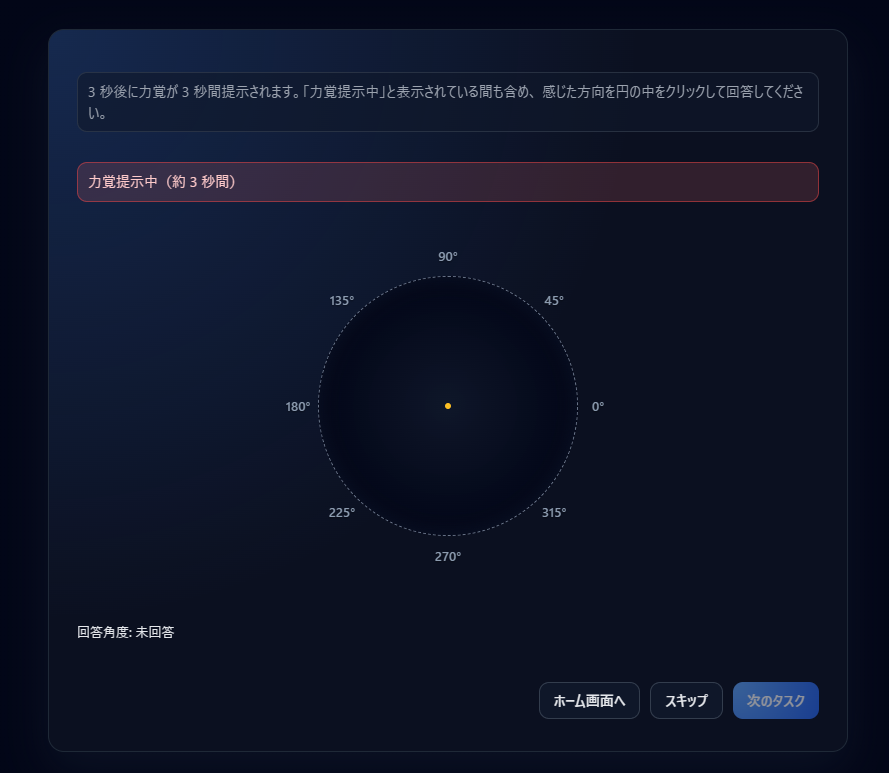
\includegraphics[width=0.85\textwidth]{figure/answer-panel.png}
\end{center}
\caption{Webアプリの回答用画面}
\label{fig:answer-panel}
\end{figure}

\begin{figure}[htbp]
\begin{center}
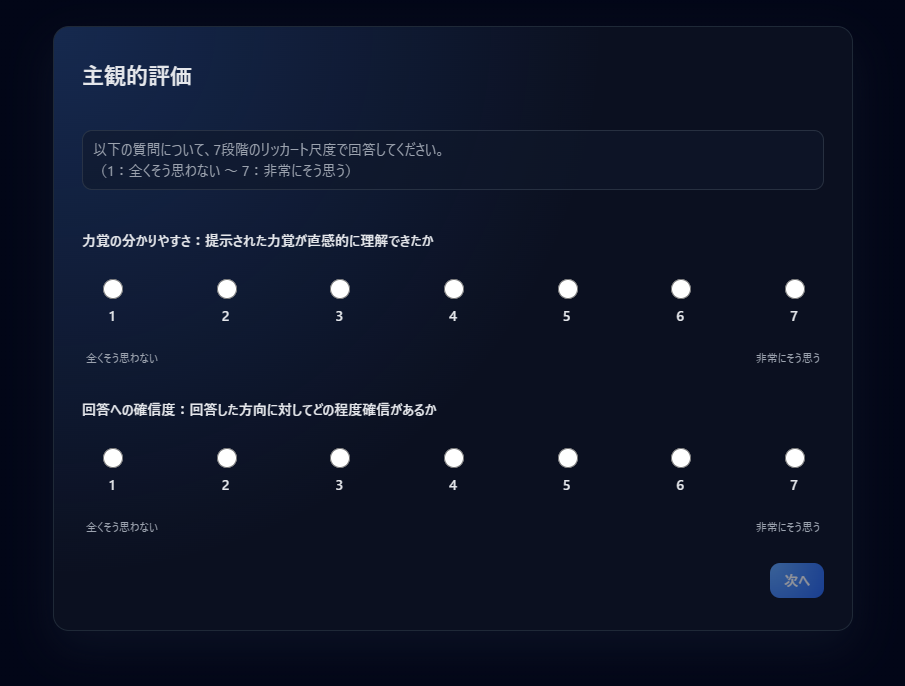
\includegraphics[width=0.85\textwidth]{figure/questionnaire-panel.png}
\end{center}
\caption{7点リッカート尺度の小質問回答画面}
\label{fig:questionnaire-panel}
\end{figure}

\begin{table}[htbp]
\begin{center}
\caption{7点リッカート尺度の小質問の内容}
\label{tab:questionnaire-items}
\begin{tabular}{c|c}
\hline
\textbf{項目} & \textbf{内容} \\
\hline
力覚の分かりやすさ & 提示された力覚が直感的に理解できたか \\
回答への確信度 & 回答した方向に対してどの程度確信があるか \\
\hline
\end{tabular}
\end{center}
\end{table}

\FloatBarrier

\section{実験環境}
実験環境を図\ref{fig:experiment-environment}に示す．実験は，ラップトップコンピュータ ThinkPad X280（CPU: Intel Core i7-8550U，メモリ：8GB，OS: Windows 10）を用いて実施した．また，実装デバイスを参加者が視認することで知覚特性に影響を与えないために，デバイスを隠す仕切り板を設置した．参加者はラップトップコンピュータの正面に着席し，各条件の装着方法に応じてデバイスを利き手に装着し，仕切り板の背後に提案デバイスを配置して実験を行った．実験者は，同室にて参加者の視界に入らない位置からシステムの監視を行った．ただし，タスク実施前後のデバイスとの接続確認時やタスク実施ログの保存時には，実験者がコンピュータを直接操作した．

\begin{figure}[htbp]
\begin{center}
\begin{minipage}{0.48\textwidth}
\centering
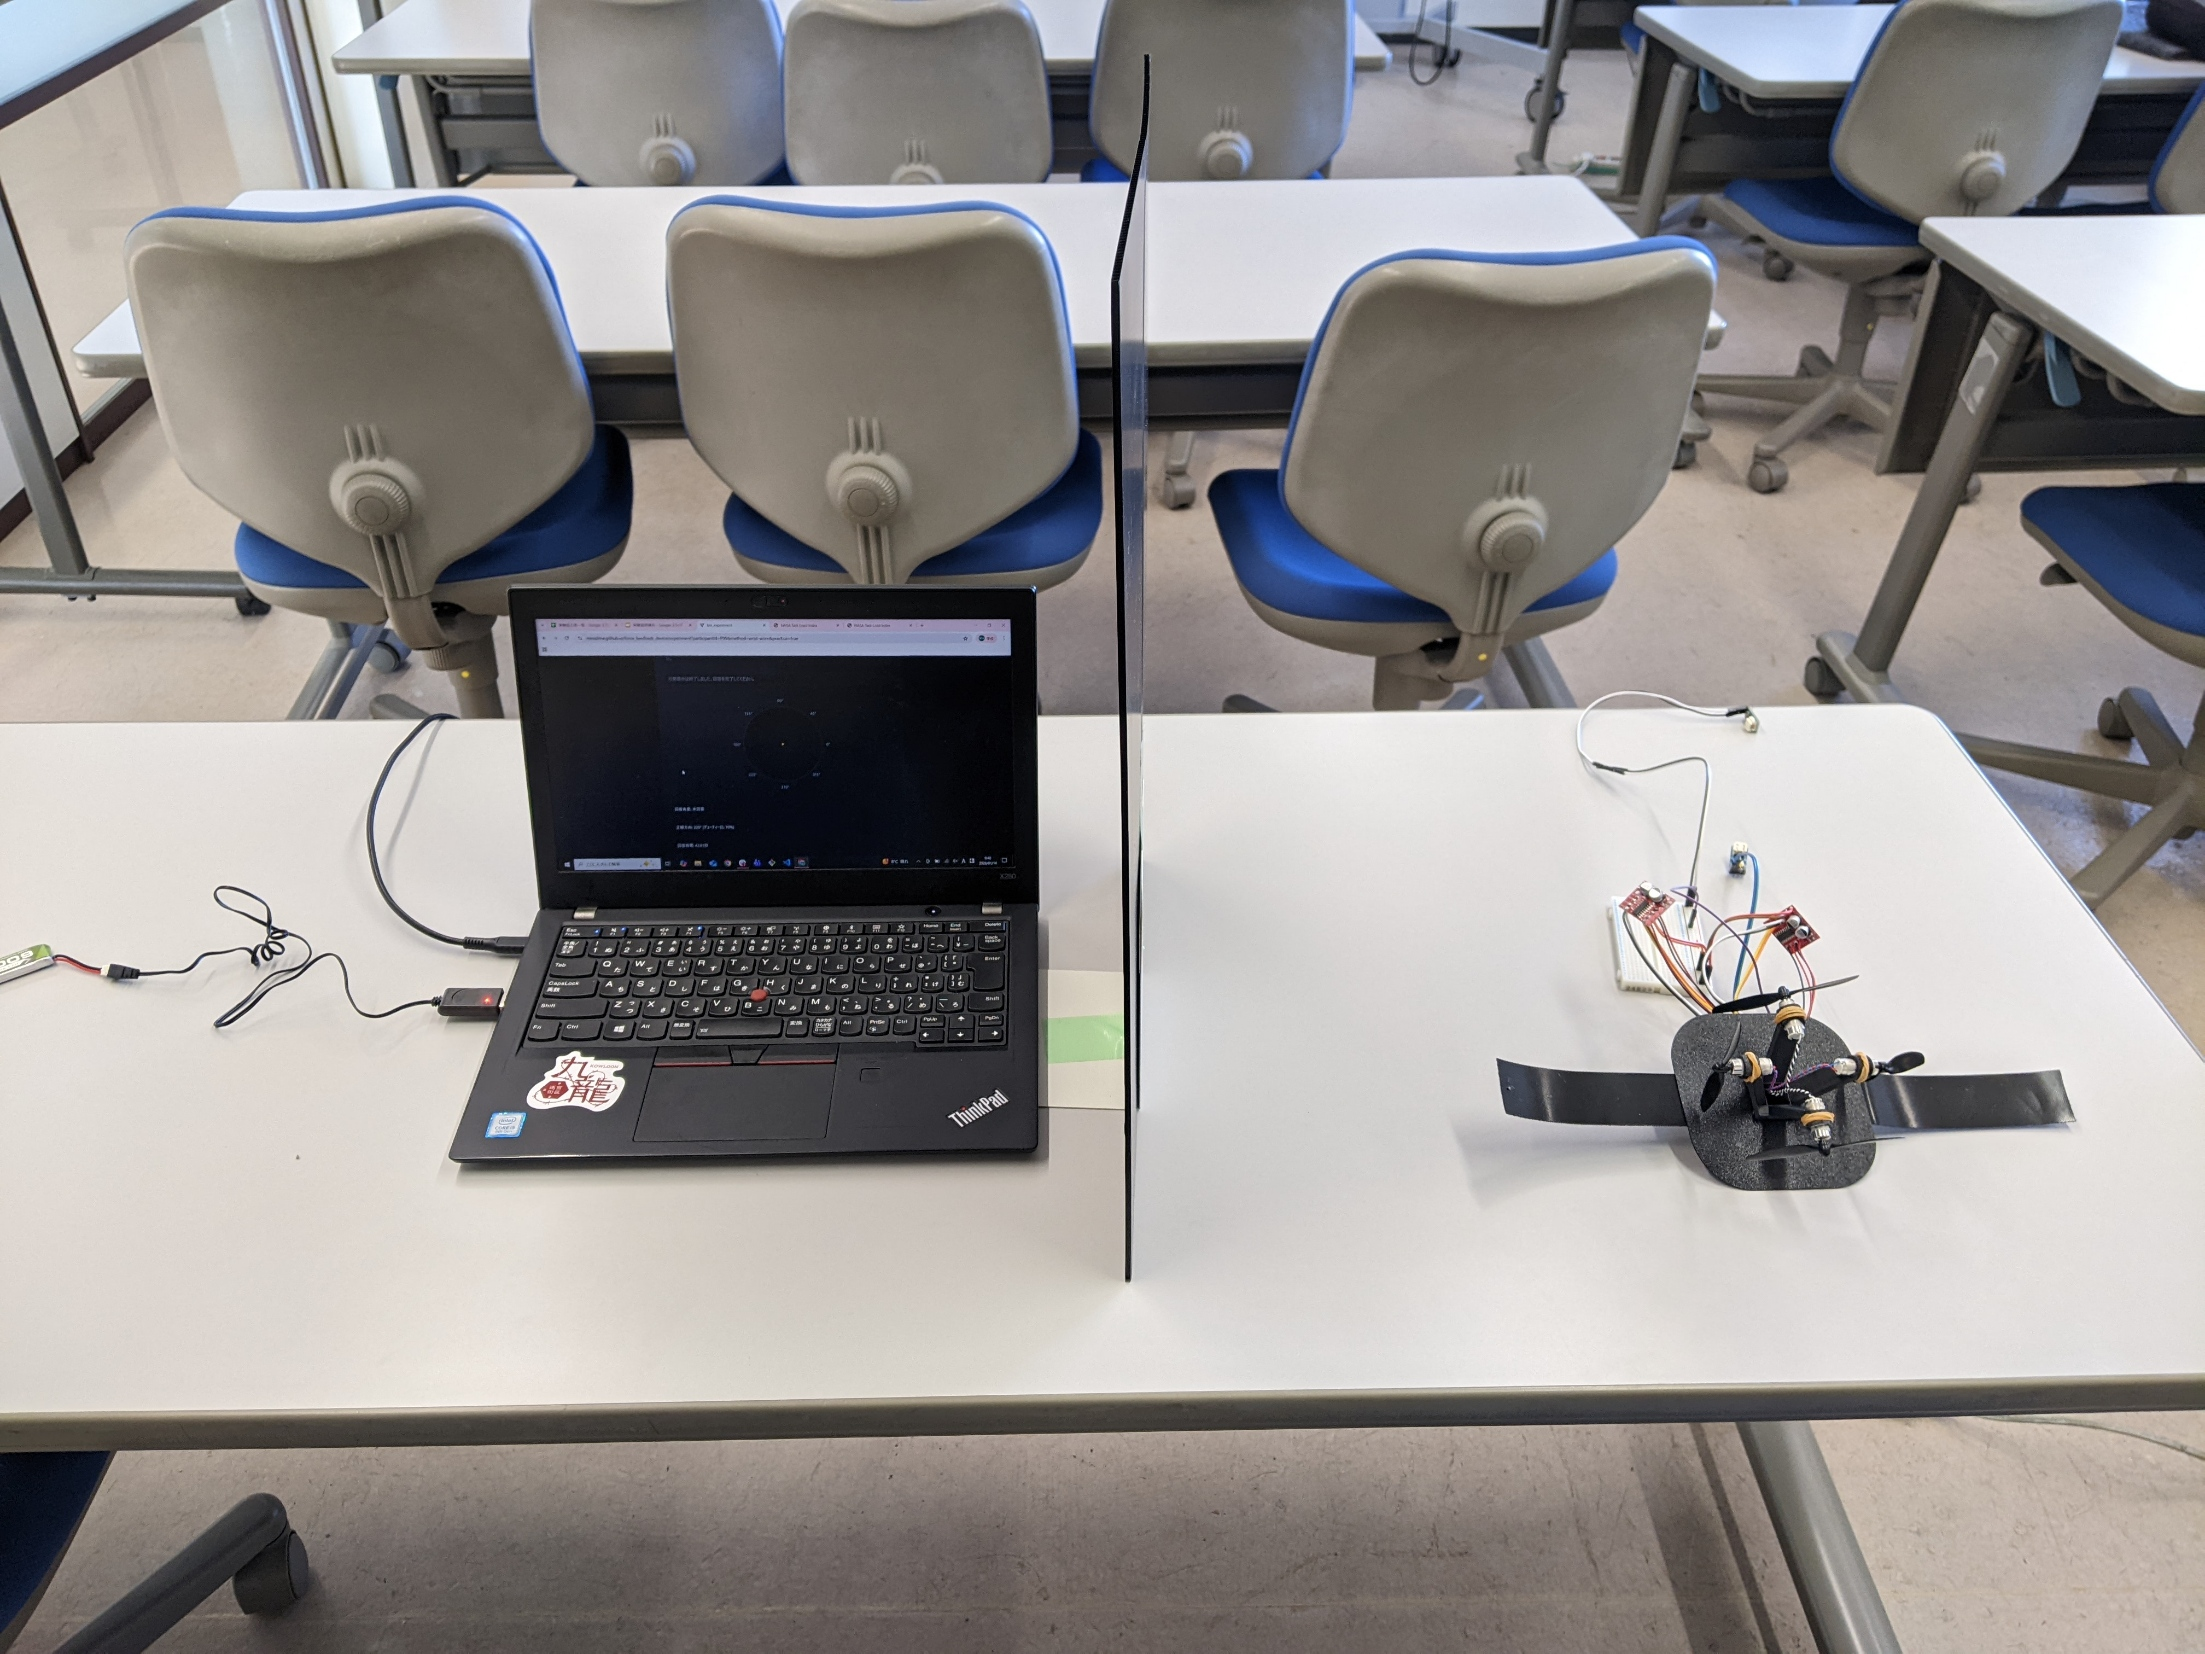
\includegraphics[width=\textwidth]{figure/experiment-environment1.jpg}
\par (a) 実験環境
\end{minipage}
\hfill
\begin{minipage}{0.48\textwidth}
\centering
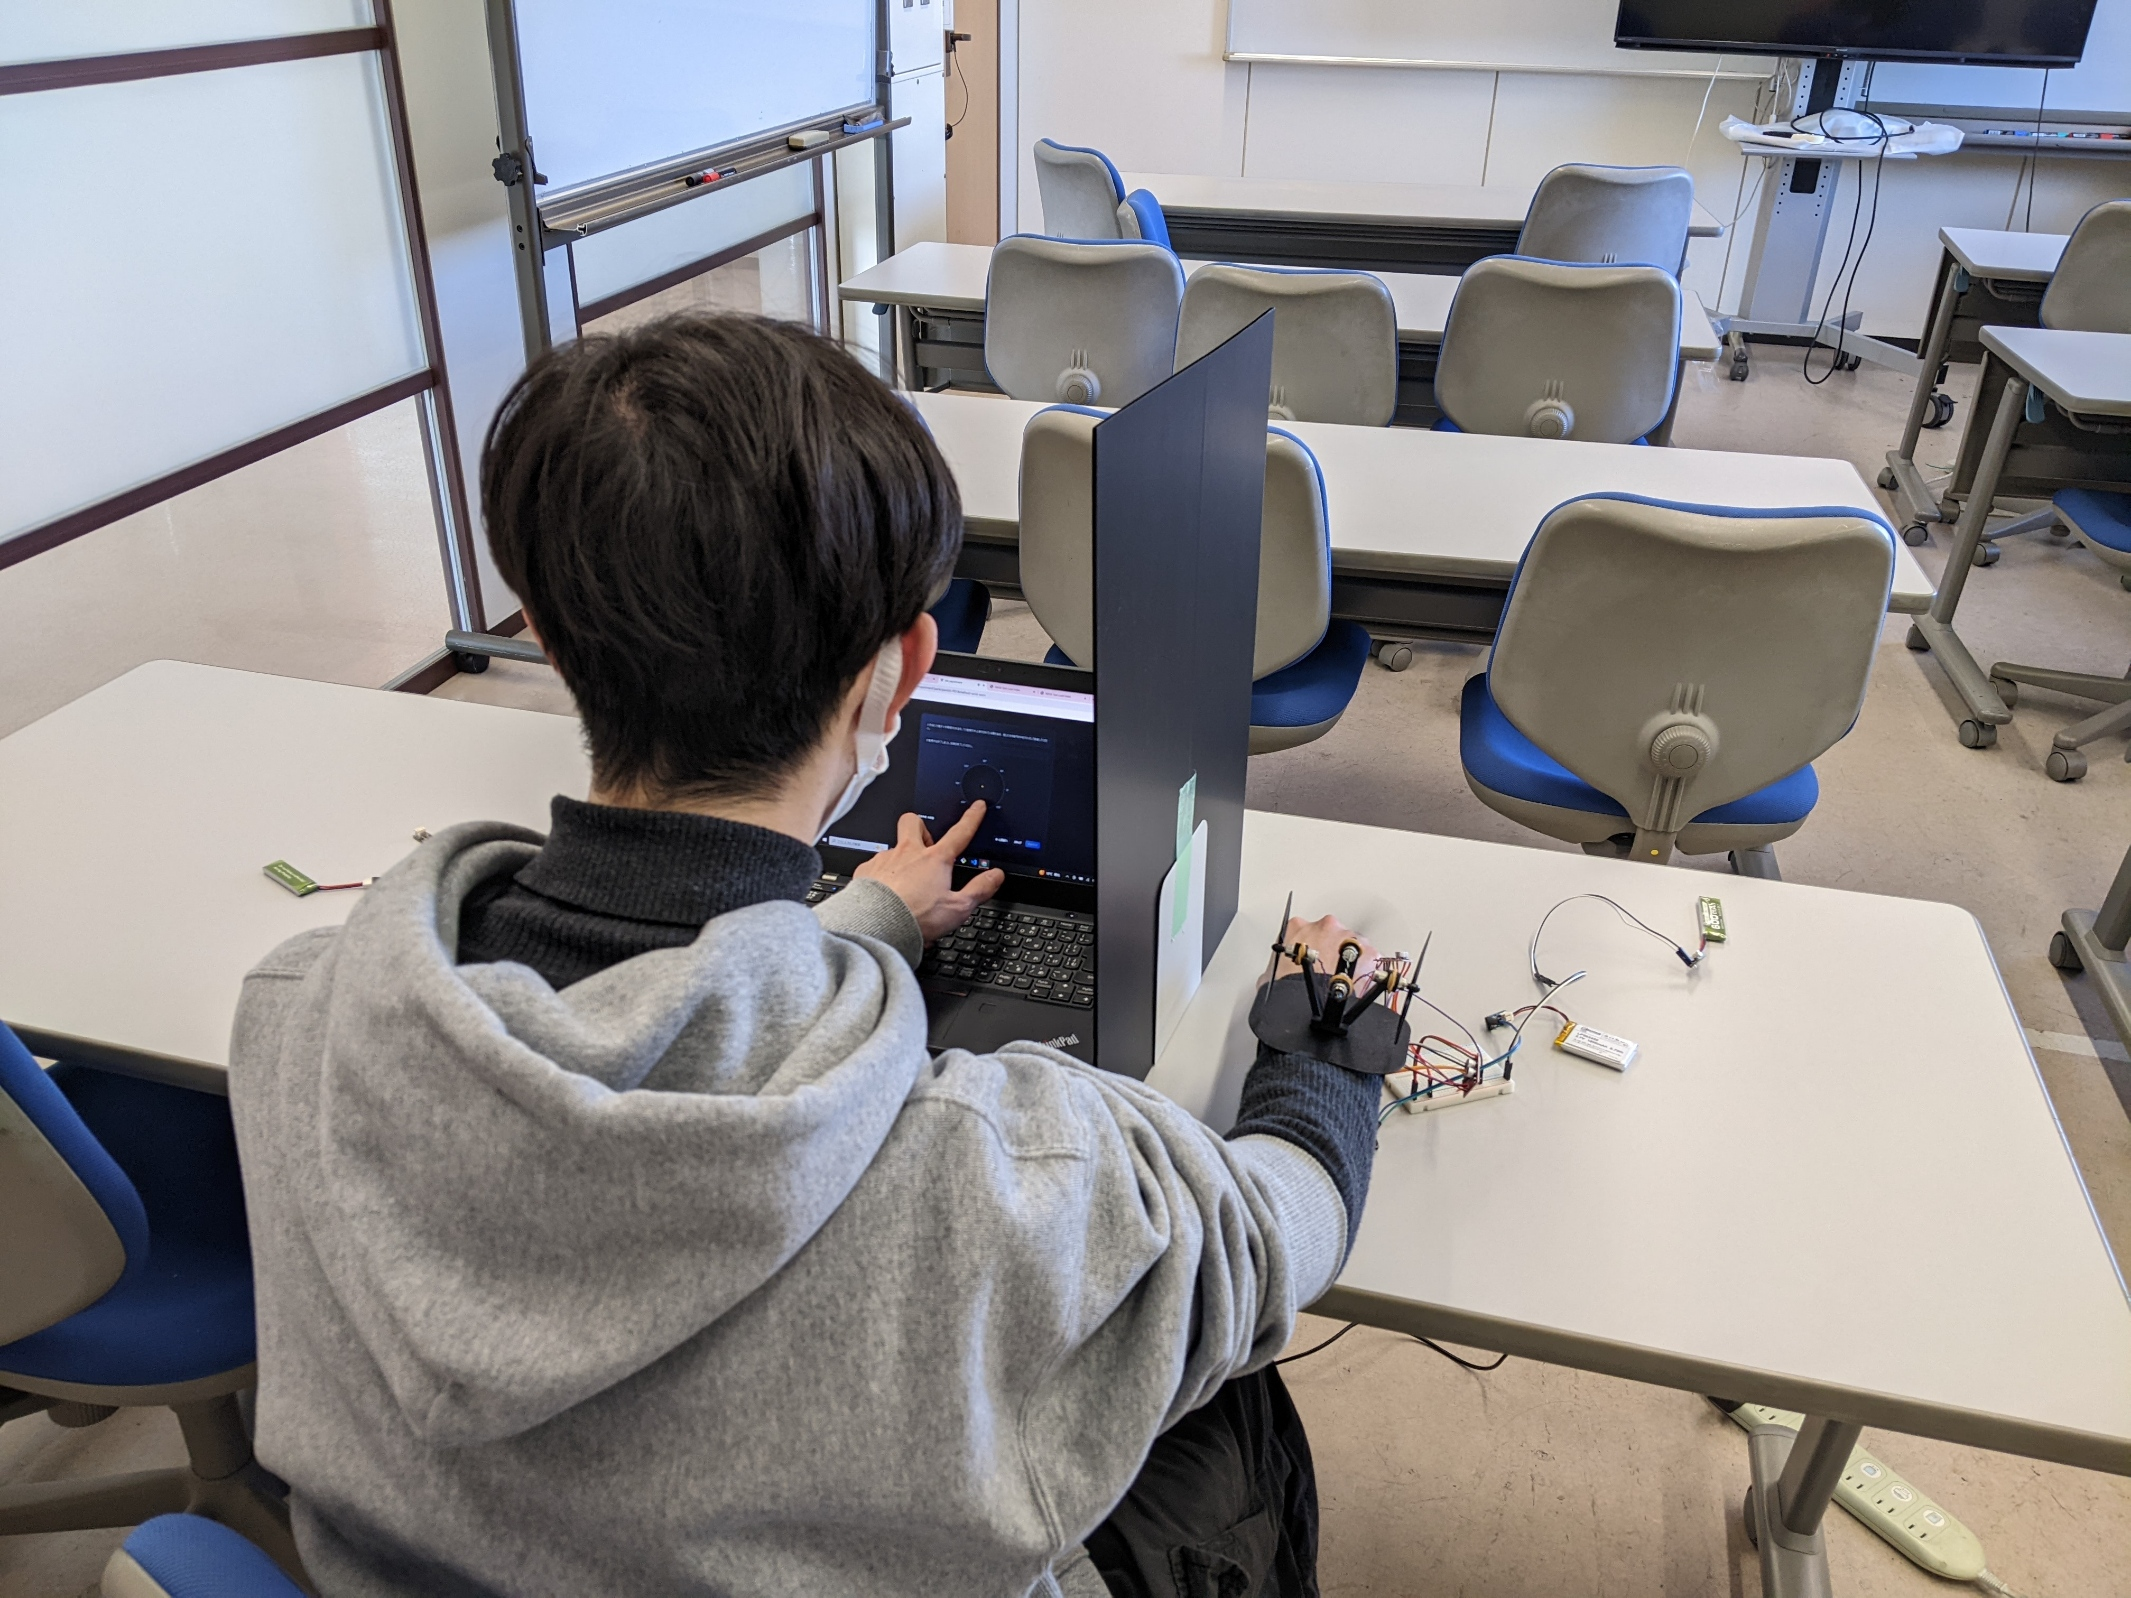
\includegraphics[width=\textwidth]{figure/experiment-environment2.jpg}
\par (b) 実験を実施している様子
\end{minipage}
\end{center}
\caption{実験環境}
\label{fig:experiment-environment}
\end{figure}

\section{実験参加者}
実験参加者は計10名（男性8名，女性2名，平均21.2歳，標準偏差0.79歳，右利き10名）の大学生である．実験は参加者内配置で行い，各参加者に対して2条件を実施した．実験全体の所用時間は45分程度であった．

\section{実験手順}
実験では，最初にシステムの説明，タスクの説明，注意事項の説明を行った．このとき，参加者にはデバイスから提示される方向の種類が8方向であることは伝えず，自身が知覚した方向を正確に回答するように指示した．続いて，実験前アンケートを実施した．その後，参加者は，提案システムを装着しながら\ref{sec:experiment-task}節で述べたタスクを行った．ここで，実験参加者のうち，参加者IDが奇数の参加者はwrist-worn条件，参加者IDが偶数の参加者はhand-grip条件を先に実施した．そして，それぞれの条件に対して，タスク終了後に作業負荷調査のためのNASA Task Load Index(NASA-TLX)\cite{nasa-tlx}を実施した．最後に，全ての条件が終了した後に実験全体に対するアンケートを行った．

タスクに対するアンケート，および実験全体に対するアンケートの具体的な内容を，付録\ref{appendix:questionnaire}として掲載する．

\section{評価指標}
各条件において，提案システムによる力覚提示の作業負荷および方向知覚特性を評価するため，以下の3つの指標を用いた．
\subsection{NASA-TLX}
システムの作業負荷を評価するために，NASA-TLXを用いた．NASA-TLXでは，知的・知覚的要求，身体的要求，時間的要求，作業成績，努力，フラストレーションの 6 つの尺度を用いてワークロードを評価する．評価は 0 から 100 の範囲で 5 点刻みの 21 段階で行い，さらに各尺度の重要度を一対比較して加重平均を算出することで，総合的な作業負荷スコアを導出する．本実験では，表\ref{table:nasa-tlx}に示す質問項目を用いて評価を実施した．

\begin{table}[hbt]
\caption{ 本実験にて利用した NASA-TLX の質問項目．}
\label{table:nasa-tlx}
\begin{center}
\begin{tabular}{ c | p{11cm} }
\hline
 & 質問項目\\
\hline
\hline
知的・知覚的要求 & どの程度の知的・知覚的活動（考える，決める，計算する，記憶する，見るなど）を必要としましたか．課題はやさしかったですか難しかったですか，単純でしたか複雑でしたか，正確さが求められましたか大ざっぱでよかったですか \\
\hline
身体的要求 & どの程度の身体的活動（押す，引く，回す，制御する，動き回るなど）を必要としましたか．作業はラクでしたかキツかったですか，ゆっくりできましたかキビキビやらなければなりませんでしたか，休み休みできましたか働きづめでしたか \\
\hline
タイムプレッシャー & 仕事のペースや課題が発生する頻度のために感じる時間的切迫感はどの程度でしたか．ペースはゆっくりとして余裕があるものでしたか，それとも速くて余裕のないものでしたか \\
\hline
作業成績 & 作業指示者（またはあなた自身）によって設定された課題の目標をどの程度達成できたと思いますか．目標の達成に関して自分の作業成績にどの程度満足していますか \\
\hline 
努力 & 作業成績のレベルを達成・維持するために，精神的・身体的にどの程度いっしょうけんめいに作業しなければなりませんでしたか \\
\hline 
フラストレーション &  作業中に，不安感，落胆，いらいら，ストレス，悩みをどの程度感じましたか．あるいは逆に，安心感，満足感，充足感，楽しさ，リラックスをどの程度感じましたか \\
\hline 
\end{tabular}
\end{center}
\end{table}

\subsection{客観的評価}
提案システムによる力覚提示の方向知覚特性を評価するため，各条件のタスク試行において，以下の2つの指標を用いた．

\begin{itemize}
    \item \textbf{誤差} 正解方向と回答角度の差（絶対誤差、度単位、360度の循環を考慮）
    \item \textbf{正答率} 誤差が一定の閾値（30度）以内の試行の割合
\end{itemize}

\subsection{主観的評価}
提案システムによる力覚提示の方向知覚特性を評価するため，各条件のタスク試行において，以下の2つの指標について，7点リッカート尺度（1: 全くそう思わない ～ 7: 非常にそう思う）を用いて評価を行った．

\begin{itemize}
    \item \textbf{力覚の分かりやすさ} 提示された力覚が直感的に理解できたか
    \item \textbf{回答への確信度} 回答した方向に対してどの程度確信があるか
\end{itemize}

また，実験終了時に，より好ましいと感じた条件を選択させ，その理由について任意で記述するアンケートを実施した．最後に，実験や提案システム全体に対する意見について任意で記述するアンケートを実施した．

\chapter{実験結果および考察}
あああ

\chapter{本研究の制約および今後の課題}
結果の解釈、限界、今後の課題を述べる。

\chapter{おわりに}
本研究の結論を述べる．

\chapter*{謝辞}
\addcontentsline{toc}{chapter}{\numberline{}謝辞}
指導教員や協力者への謝辞を記述する。

\newpage
\addcontentsline{toc}{chapter}{\numberline{}参考文献}
\renewcommand{\bibname}{参考文献}
\bibliographystyle{unsrt}
\bibliography{references}

\appendix
\chapter{実験にて使用したアンケート}
\label{appendix:questionnaire}
実験にて使用したアンケートの具体的な内容を以下に示す．

\newpage

\section{実験前アンケート}
\begin{figure}[htbp]
\begin{center}
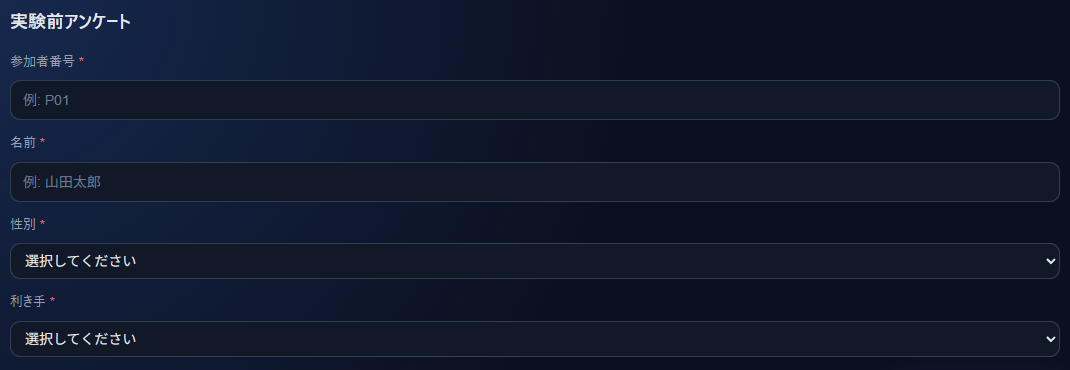
\includegraphics[width=0.85\textwidth]{figure/questionnaire1.png}
\end{center}
\label{fig:pre-questionnaire}
\end{figure}

\newpage

\section{実験後アンケート}
\begin{figure}[htbp]
\begin{center}
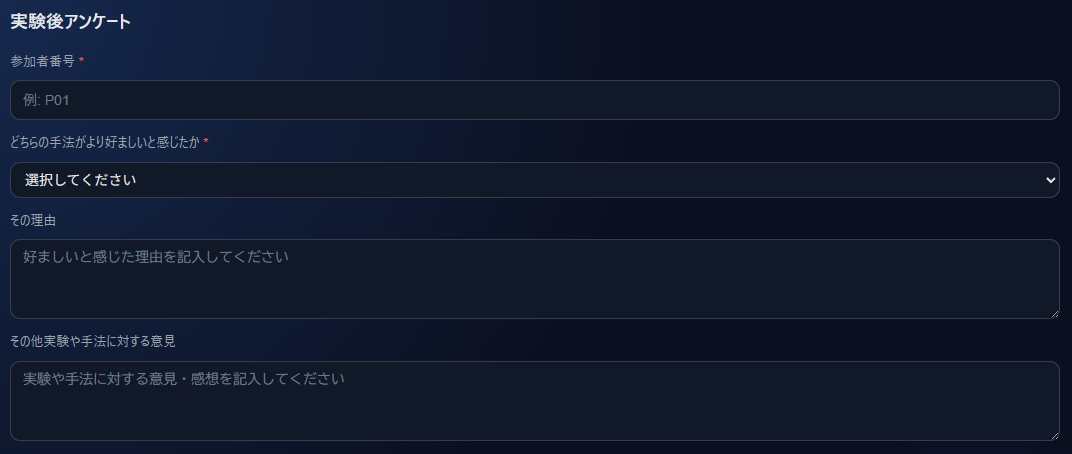
\includegraphics[width=0.85\textwidth]{figure/questionnaire2.png}
\end{center}
\label{fig:post-questionnaire}
\end{figure}
\end{document}
